\section*{Pregunta 4}
\noindent Describe una secuencia de accesos a un árbol splay $T$ de $n$ nodos, con $n \geq 5$ impar, que resulte en $T$ siendo una sola cadena de nodos en la que el camino para bajar en el árbol alterne entre hijo izquierdo e hijo derecho.

\subsection*{Respuesta}

La secuencia es 7,10,13,15,17 y podemos ver los accesos en la siguiente figura
\begin{figure}
    \centering
    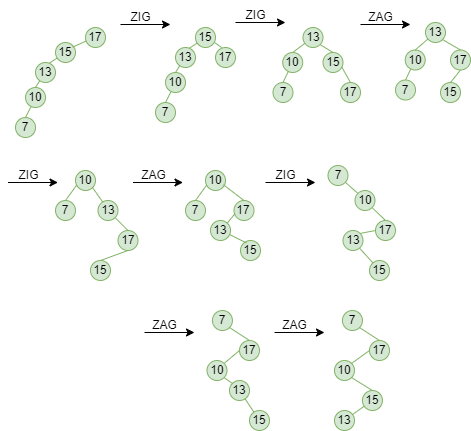
\includegraphics[width=\textwidth]{t1-4.png}
\end{figure}

\bigskip
